\newpage
\slidetitle{}
\section{Einleitung}
\begin{center}
	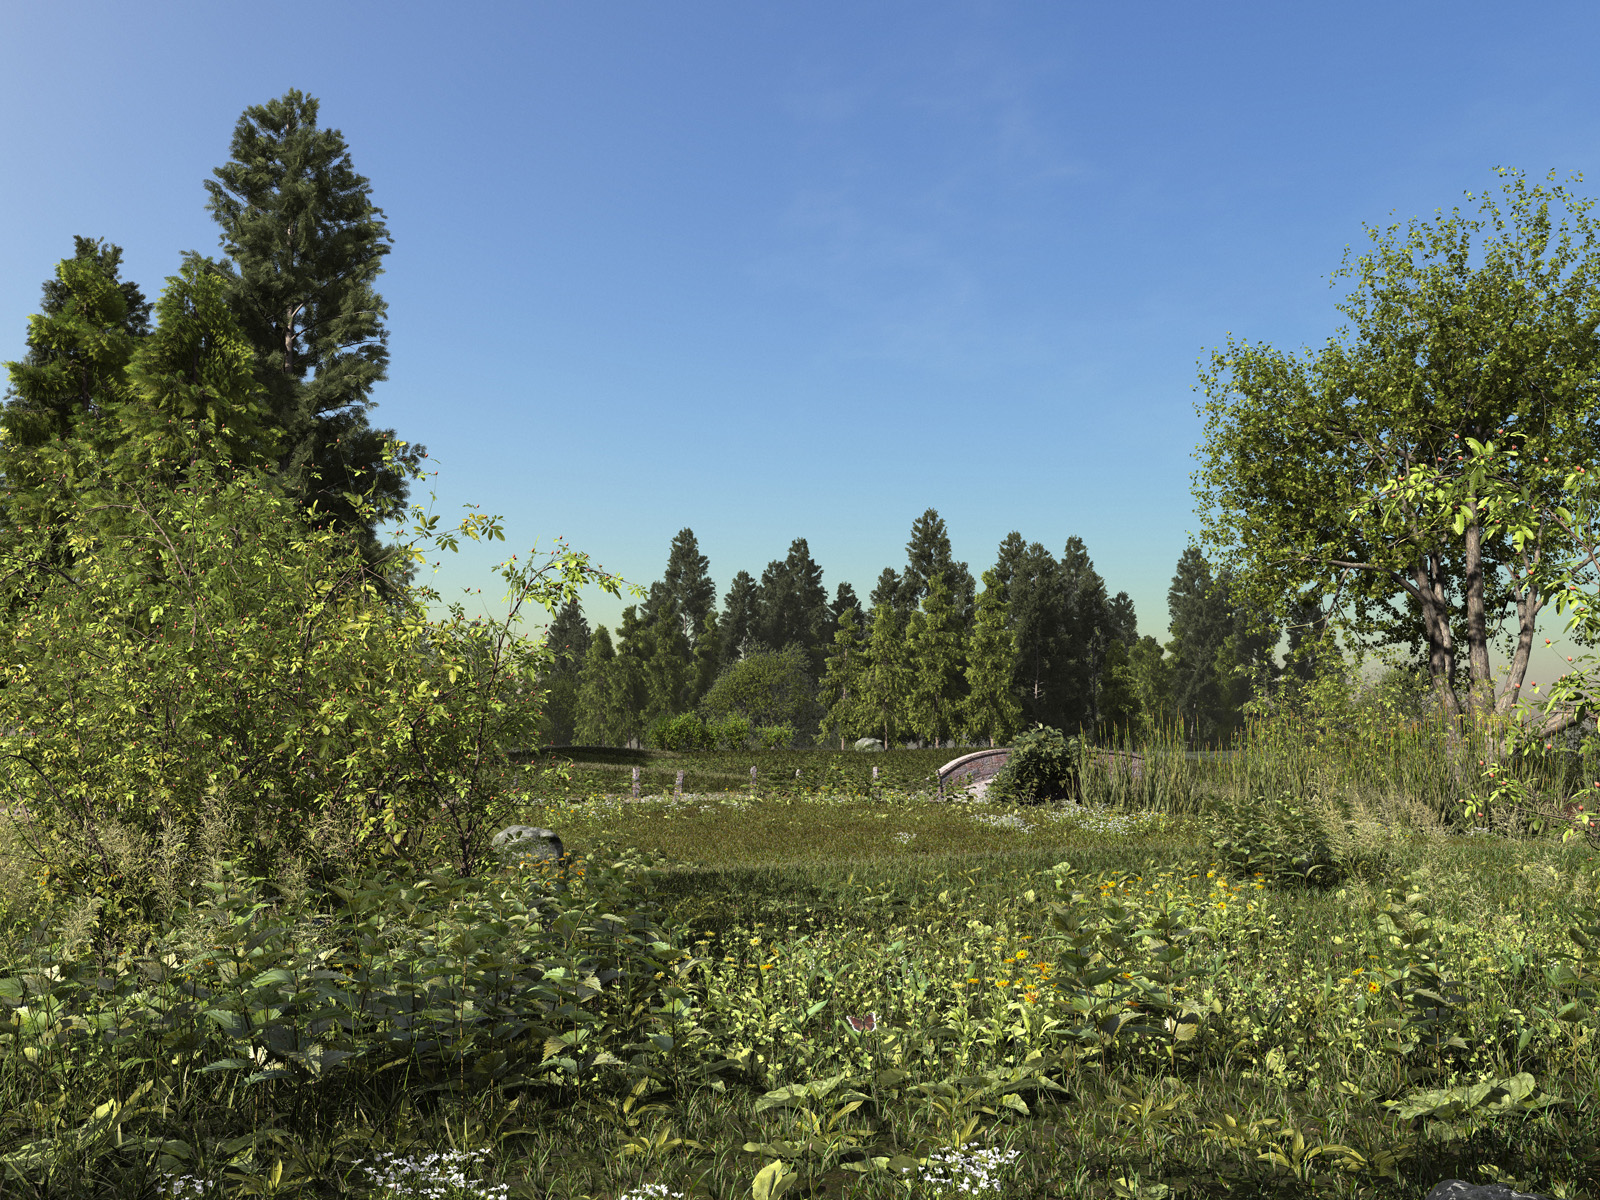
\includegraphics[height=.85\textheight]{images/CH1_greenXfrog_JanWalterSchliep.jpg}
	\cite{GreenOne:16}
\end{center}

%\paragraph{Prozedurale Generierung\\}
%\begin{itemize}
%	\item Konstruktion von 3D-Modellen mithilfe computergenerierter Daten\\
	
%	\item Benötigt lediglich eingeschränkten Eingriff durch Benutzer\\
	
%	\item Generierung von Pflanzenmodellen
%\end{itemize}


\newpage
\slidetitle{1. Einleitung - Ansatz}
\paragraph{Ansatz\\}

\begin{itemize}
	\item Implementierung von zwei Verfahren zur prozeduralen Generierung von Baumstrukturen:
	\begin{itemize}
		\item Lindenmayer-Systeme
		\item Space Colonization Algorithmus\\
	\end{itemize}
	\item Verwendung des Frameworks \glqq Unreal Engine 4\grqq\\
	
	\item Vereinfachte Darstellung von Ästen in Form von Zylindern
\end{itemize}

\newpage
\slidetitle{1. Einleitung - Unreal Engine 4}
\paragraph{Unreal Engine 4\\}

\begin{itemize}
	\item Sammlung von Softwarewerkzeugen \\
	
	\item Erstellung von Inhalten mit C++ oder Blueprint und auf Basis von Framework-Klassen\\
	
	\item Verfügbarkeit eines visuellen Editor erlaubt:
	\begin{itemize}
		\item Einfache Positionierung von Actors
		\item Eingabe von Parametern über das Editor-UI
	\end{itemize}
\end{itemize}

\iffalse

\newpage
\begin{center}
	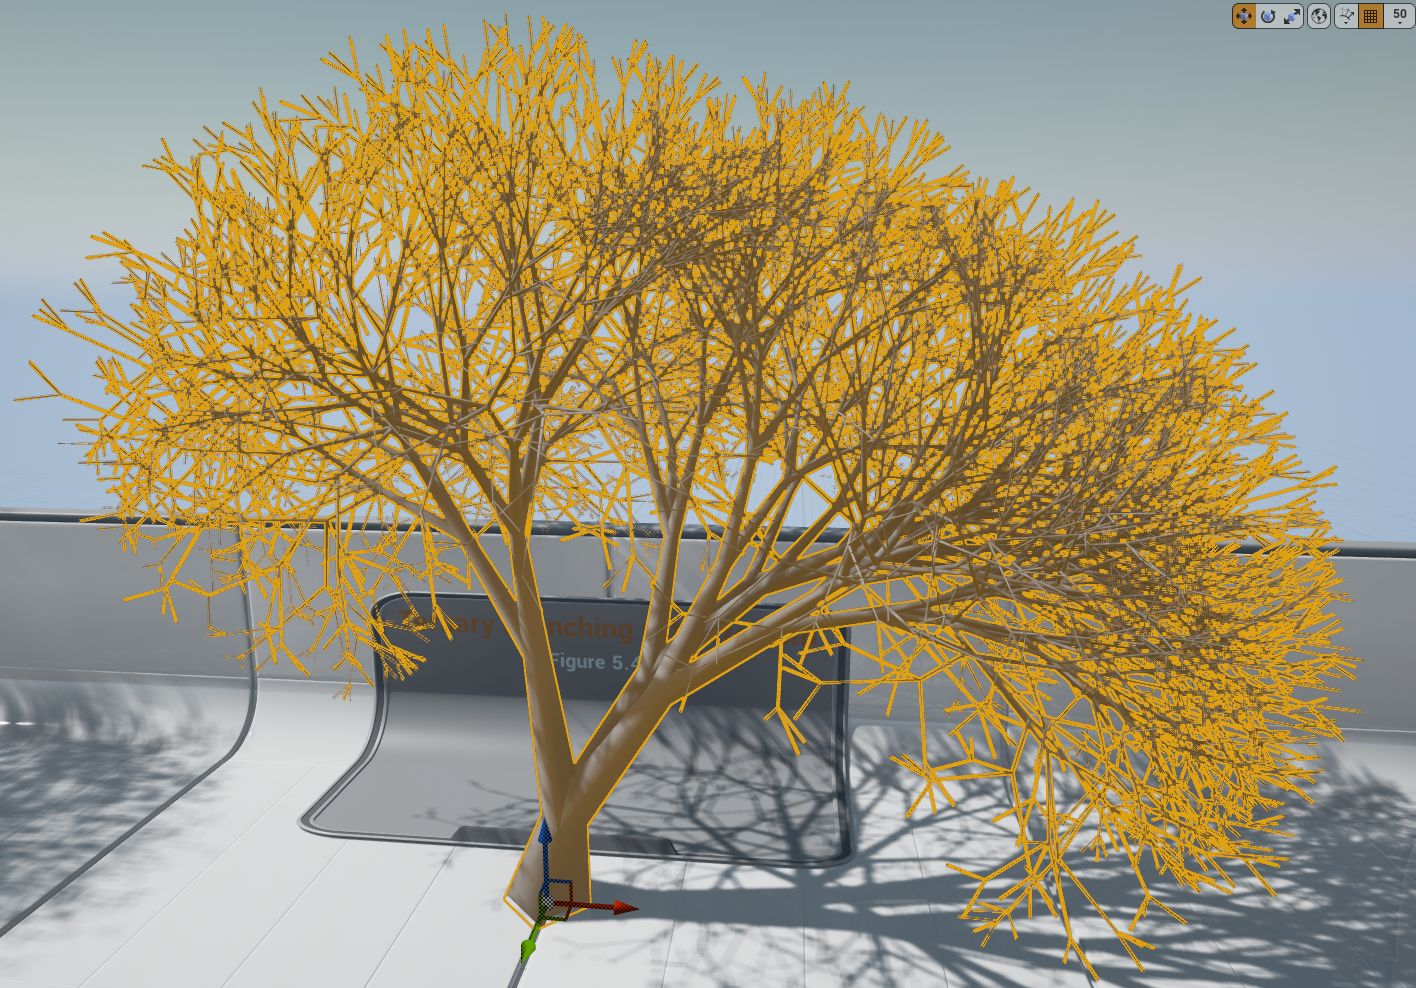
\includegraphics[height=0.9\textheight]{images/CH1_EditorExample1.png}
	
	Positionierung eines Actors im Leveleditor
\end{center}

\begin{center}
	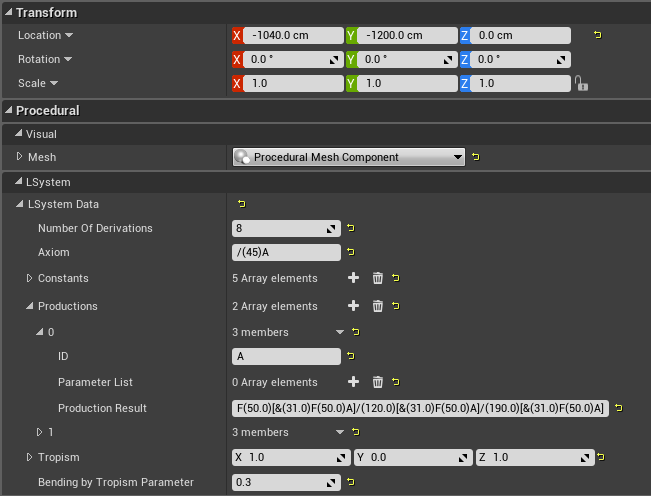
\includegraphics[height=0.9\textheight]{images/CH1_EditorExample2.png}
	
	Eingabefenster für Actor-Parameter
\end{center}



\newpage
\slidetitle{1. Einleitung - Bisherige Arbeiten}
\paragraph{Bisherige Arbeiten}
\begin{center}
	\begin{minipage}[c]{0.45\textwidth}
		\centering
		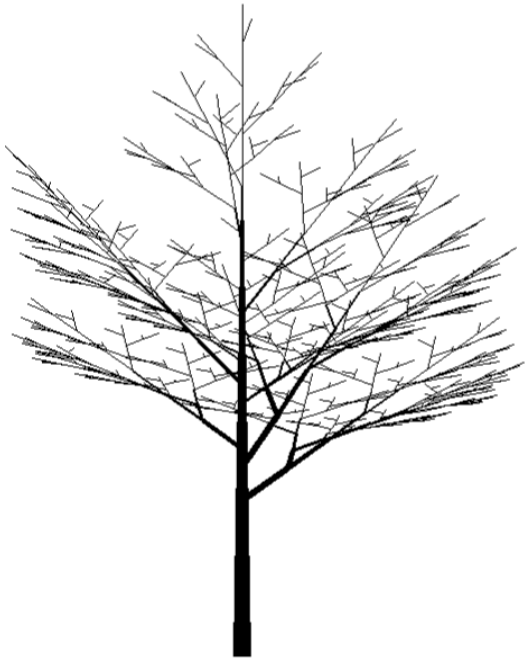
\includegraphics[height=0.6\textheight]{images/CH1_Honda1.png}
		
		Honda und Fisher \cite{ABOP:04}
	\end{minipage}
	\hspace{.05\textwidth}	
	\begin{minipage}[c]{0.45\textwidth}
		\centering
		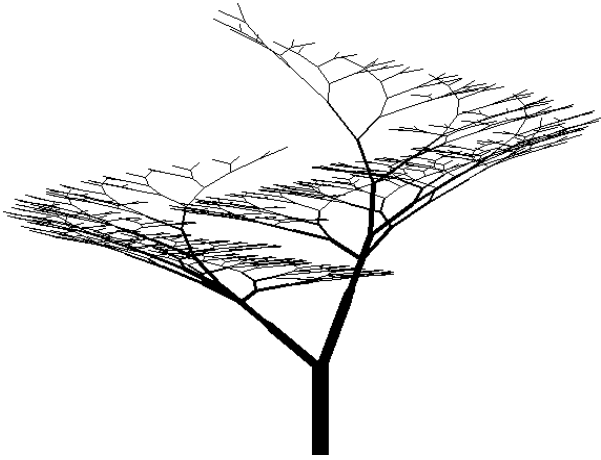
\includegraphics[height=0.6\textheight]{images/CH1_AonoKunii1.png}
		
		Aono und Kunii \cite{ABOP:04}
	\end{minipage}
\end{center}


\begin{center}
	\vfill
	\begin{minipage}[c]{0.45\textwidth}
		\centering
		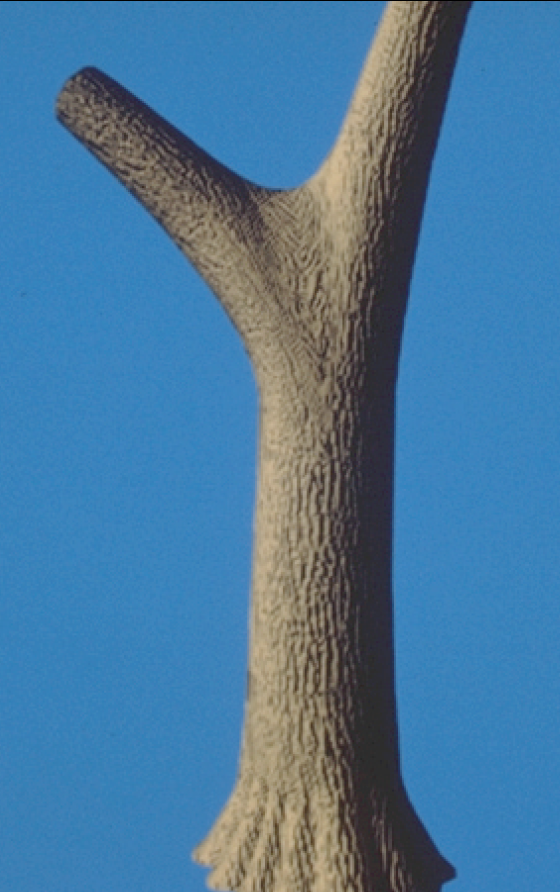
\includegraphics[height=0.6\textheight]{images/CH1_Bloomenthal1.png}
		
		Bloomenthal \cite{ABOP:04}
	\end{minipage}
	\hspace{.05\textwidth}	
	\begin{minipage}[c]{0.45\textwidth}
		\centering
		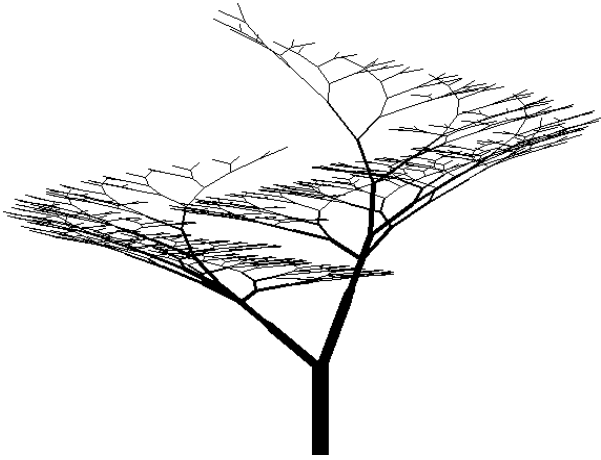
\includegraphics[height=0.6\textheight]{images/CH1_AonoKunii1.png}
		
		Aono und Kunii \cite{ABOP:04}
	\end{minipage}
\end{center}
\fi


	